\documentclass{beamer}
\DeclareFontShape{OT1}{cmss}{b}{n}{<->ssub * cmss/bx/n}{} 
\usetheme{default}
\usepackage{amsmath}
\usepackage{amsfonts}
\usepackage{mathbbol}
\usepackage{xcolor} % before tikz or tkz-euclide if necessary
\usepackage{tkz-euclide} % no need to load TikZ
\usepackage{multirow}
\usepackage{lmodern}
\usepackage{bm}
\usepackage{hyperref}
\usepackage{subfigure}

\titlegraphic{\includegraphics[width=2cm]{../../Figures/UAMS_RGB.png}
}


\title{Single-Cell RNA-seq Analysis\\ Methods Overview}
\author{Horacio G\'omez-Acevedo\\ Department of Biomedical Informatics\\
	University of Arkansas for Medical Sciences}
\begin{document}
	\begin{frame}[plain]
		\maketitle
	\end{frame}
	\begin{frame}{sc-RNA seq}
		
\begin{figure}[h]
	\centering
	\includegraphics[scale=0.25]{../../Figures/scrnaseq_overview.png}
	\caption{\href{https://github.com/theislab/single-cell-tutorial}{Overview}}
\end{figure}
\end{frame}

\begin{frame}{Bulk vs Single-cell RNAseq}
	
\begin{figure}%
	\centering
	\subfigure[ Bulk RNAseq]{\includegraphics[scale=0.4]{../../Figures/bulk_rnaseq.png} }%
	\qquad
	\subfigure[ Sc-RNAseq]{\includegraphics[scale=0.4]{../../Figures/sc_rnaseq.png} }%
%	\caption{2 Figures side by side}%
%	\label{fig:example}%
\end{figure}
	
\end{frame}

	
	\begin{frame}{Space: the final frontier}
		
The mathematical representation of the data is given by placing the readings (RPKM) of each individual gene in an "axis" of an $n$ dimensional space.
 In this case $n$ represents a large number of genes.
 
\begin{figure}[h]
	\centering
	\includegraphics[scale=0.45]{../../Figures/sc_space.png}
	\caption{Spatial representation of scRNAseq data}
\end{figure}
		
	\end{frame}
	
\begin{frame}{PCA interlude}

Principal Component Analysis is one of the most commonly used methodologies to "inspect" high dimensional data. 

\begin{figure}[h]
	\centering
	\includegraphics[scale=0.45]{../../Figures/sc_space1.png}
	\caption{Plane projection of data}
\end{figure}	
	
\end{frame}	

\begin{frame}{PCA projection}
	The main goal of PCA  is to find the representation of our data in a lower dimensional space (mostly a plane). But the selection of such plane should preserve original data variability. 
	
	Formally, the two directions represent the directions of the maximal variability of our data. 

\end{frame}	

\begin{frame}{RGB example}
\begin{figure}[h]
	\centering
	\includegraphics[scale=0.45]{../../Figures/pca_rgb.png}
	\caption{Plane projection of RGB data}
\end{figure}		


\end{frame}	

\begin{frame}{Clustering}
	Clustering refers to a set of computational techniques for finding subsets or {\sl clusters} in a data set.  Clustering is among the so-called {\bf unsupervised learning methodologies } .\\
	
	\begin{center}
		Unsupervised $\ne$ Automatic
	\end{center}
	
	Thus, the main goal of clustering is to find homogeneous subgroups among the data. 
		
\end{frame}
	
\begin{frame}{Clustering terminology}
	


Let's define a distance between two points (in a plane), say $d$. Also, the {\sl centroid } of a cluster is the mean of their observations.

\begin{figure}[h]
	\centering
	\includegraphics[scale=0.65]{../../Figures/centroid.png}
	\caption{Distance and Centroid of a cluster}
\end{figure}	
\end{frame}

\begin{frame}{K-means clustering}
One of the simplest methods for clustering is $K$-means clustering. 

We begin with a data set and a value $K$ fixed by a human (say $K=3$). 

\begin{enumerate}
	\item Assign randomly a value between 1 and K to each data point.
	\item Iterate the following procedure until the clusters assignments stop changing 
	\begin{enumerate}
		\item Find the centroid for each of the $K$ clusters.
		\item Each point will be assigned to the cluster $K$ whose distance is the smallest. If two or more are equidistant, select randomly the cluster among the equidistant clusters.
	\end{enumerate}	
\end{enumerate}


\end{frame}

\begin{frame}{K-means clustering picture}
	
	\begin{figure}[h]
		\centering
		\includegraphics[scale=0.55]{../../Figures/kmeans_clustering.png}
		%\caption{Distance and Centroid of a cluster}
	\end{figure}	
	\href{https://www.statlearning.com/}{An Introduction to Statistical Learning (Chapter 10)}
\end{frame}

\begin{frame}{Problems with K-means clustering}
	\begin{itemize}

		\item Selection of the distance function $d$ (Euclidean, Pearson correlation, arccos, etc.) 
		\item Selection of $K$.
	\end{itemize}
	\begin{figure}[h]
	\centering
	\includegraphics[scale=0.55]{../../Figures/kmeans_K.png}
	%\caption{Distance and Centroid of a cluster}
\end{figure}	
\href{https://www.statlearning.com/}{An Introduction to Statistical Learning (Chapter 10)}	
	
\end{frame}
	
\begin{frame}{t Stochastic Neighbor Embedding}

$t$-SNE maps a set of high-dimensional points to a plane, such that ideally, close neighbors remain close and distant points remain distant.

 Informally, the algorithm places all
points on the 2D plane, initially at random positions, and lets them
interact as if they were physical particles. 

The interaction is governed
by two laws: 
\begin{itemize} 
	\item all points are repelled from each other
\item each point is attracted to its nearest neighbors
\end{itemize}
This methodology is governed by a parameter called {\bf perplexity}.

\end{frame}	

\begin{frame}{tSNE vs PCA}
	A visual comparison of PCA vs tSNE
	
		\begin{figure}[h]
		\centering
		\includegraphics[scale=0.55]{../../Figures/pca_vs_tsne.png}
		%\caption{Distance and Centroid of a cluster}
	\end{figure}	
	
	
\end{frame}
	
	\begin{frame}{Out-of-Bag Observations}
		
		The main idea of the bootstrap is that from $m$ observations, we select a sample with replacement $m$ observations.
		
		What is the probability of {\bf not} selecting sample 1 ?
		
		The probability of picking sample different from 1 would be 
		$(1 - \frac{1}{m})$. Since we are repeating the experiment with replacement, the probability that a bootstrap sample does not contain sample 1 is 
		\begin{equation*}
			\left(1 - \frac{1}{m}\right) \cdot \left(1 - \frac{1}{m}\right) \cdots \left(1 - \frac{1}{m}\right) = \left(1 - \frac{1}{m}\right)^m
		\end{equation*}
		A little bit of calculus shows that 
		\begin{equation*}
			\lim_{m\to\infty}\left(1-\frac{1}{m}\right)^m= \exp(-1) \approx 36.79\%
		\end{equation*}
		Thus, bootstrapping will not touch about 1/3 of the observations!
		and those observations are referred to as {\bf Out-of-Bag (OOB)}.  
	\end{frame}
	
	\begin{frame}{OOB Error Estimation}
		We can exploit the OOB observations to estimate the test error in the bagging process without the need of cross-validation or even a split of the data in training and testing.
		
		Once we have obtained our $\hat{f}_{bag}(x)$, we can use the OOB observations (i.e., observations not used for the bagging estimation) to determine predictions. 
		
		More precisely, we obtain $\hat{f}_{\textrm{oob}}^i (x)$ based on the OOB observations $\{x_{i1},\ldots, x_{iK}\}$, where $K \approx B/3$ for $B$ big enough. 
		
		
		
		
		\begin{equation*}
			\hat{f}_{OOB}(x)= \frac{1}{K}\sum_{i=1}^{K} \hat{f}^{i}_{\textrm{oob}}(x)
		\end{equation*}
		This procedure leads to the calculation of the test MSE that is a valid estimate since the response is derived from trees that were not involved in the bagged model.
		
		A similar expression is valid for classification, but instead of the average we can use the majority vote and purity metrics instead of MSE or RSS. 
	\end{frame}
	
	
	\begin{frame}{Variable Importance Measures}
		
		We know that bagging improves the accuracy in our predictions, at the expense of making our models harder to interpret. 
		
		For bagging regression trees, we use the {\bf Variable Importance Measure (VIM)} that is defined as the total amount that the RSS is decreased due to splits over the given predictor, averaged over all $B$ trees.  The larger the VIM, the more "relevant" is that predictor.
		
		For bagging classification trees, we can define VIM as the total amount that the Gini index (or cross-entropy) is decreased by splits over a given predictor, averaged over all $B$ trees. 
	\end{frame}
	
	\begin{frame}{VIM example}
		The {\tt Heart} data set VIM plot with a mean decrease of GIni index and normalized VIM is shown below.
		\begin{figure}[h]
			\centering
			\includegraphics[scale=0.35]{../../Figures/fig_vim.png}
		\end{figure}
		
	\end{frame}
	
	\begin{frame}{Random Forest}
		It follows similar rationale as in bagging but with an interesting random twist.
		
		We build a number of decision trees on bootstrapped training samples. But when building these decision trees, each time a split in a tree is considered, a {\it random sample of $m$ predictors} is chosen as split candidates from the full set of $p$ predictors.  We normally set $m\approx \sqrt{p}$.
		
		What is the advantage of random forest over bagging?
		
		When we have a strong predictor, bagging trees will consider that predictor frequently, thus bagging trees will look alike. By having a random choice on the predictors, we may generate "different" trees that otherwise we would not have explored. This process is referred to as {\it decorrelating trees}. 
		
	\end{frame}
	
	\begin{frame}{Random Forest vs Bagging}
		The test errors from the {\tt Heart} data are depicted below
		\begin{figure}[h]
			\centering
			\includegraphics[scale=0.35]{../../Figures/fig_bagging.png}
		\end{figure}
	\end{frame}
	
	\begin{frame}{Boosting}
		
		{\bf Boosting} is another general methodology to improve the predictions from a decision tree. 
		In this case trees are grown sequentially as they gather information from previously generated trees. 
		
		Boosting does not require bootstrap sampling as each tree is fit on a modified version of the original data set.
		
		
		
	\end{frame}
	
	\begin{frame}{Boosting Algorithm}
		\begin{enumerate}
			\item Set $\hat{f}(x)=0$ and $r_i=y_i$ for all $i$ in the training set. 
			\item for $b=1,\ldots, B$ repeat:
			\begin{enumerate}
				\item Fit a tree $\hat{f}^b$ with $d$ splits to the training data $(X,r)$.
				\item Update $\hat{f}$ by adding in a shrunken version of the new tree:
				\begin{equation*}
					\hat{f}(x) \leftarrow \hat{f}(x)+ \lambda \hat{f}^b (x)
				\end{equation*}
				\item Update the residuals,
				\begin{equation*}
					r_i \leftarrow r_i - \lambda \hat{f}^b(x_i)
				\end{equation*}
			\end{enumerate}
			\item Output the boosted model
			\begin{equation}
				\hat{f}(x)=\sum_{b=1}^B \lambda \hat{f}^b(x)
			\end{equation}
		\end{enumerate}
	\end{frame}
	
	\begin{frame}{Boosting}
		Given a current model, we fit a decision tree to the residuals from the model rather than the outcome $Y$ as the response. And we add these residuals to a new decision tree and update again the residuals. 
		
		Boosting has the following tuning parameters:
		
		\begin{itemize}
			\item $B$ that represents the number of trees. Do not take very large values of $B$ as boosting tends to overfit. We can use cross-validation to determine a good candidate for $B$.
			\item The shrinkage parameter $\lambda$ controls the learning rate. 
			\item The number of splits $d$ controls the complexity of the boosted ensemble. Sometimes $d=1$ works well. 
	\end{itemize} \end{frame}
	
	
	\begin{frame}{Boosting}
		Boosting and random forest comparison in a 15-class gene expression data set to predict cancer.
		\begin{figure}[h]
			\centering
			\includegraphics[scale=0.35]{../../Figures/fig_boosting.png}
		\end{figure}
		
	\end{frame}
	
	\begin{frame}{Final Thoughts}
		
		\begin{figure}[h]
			\centering
			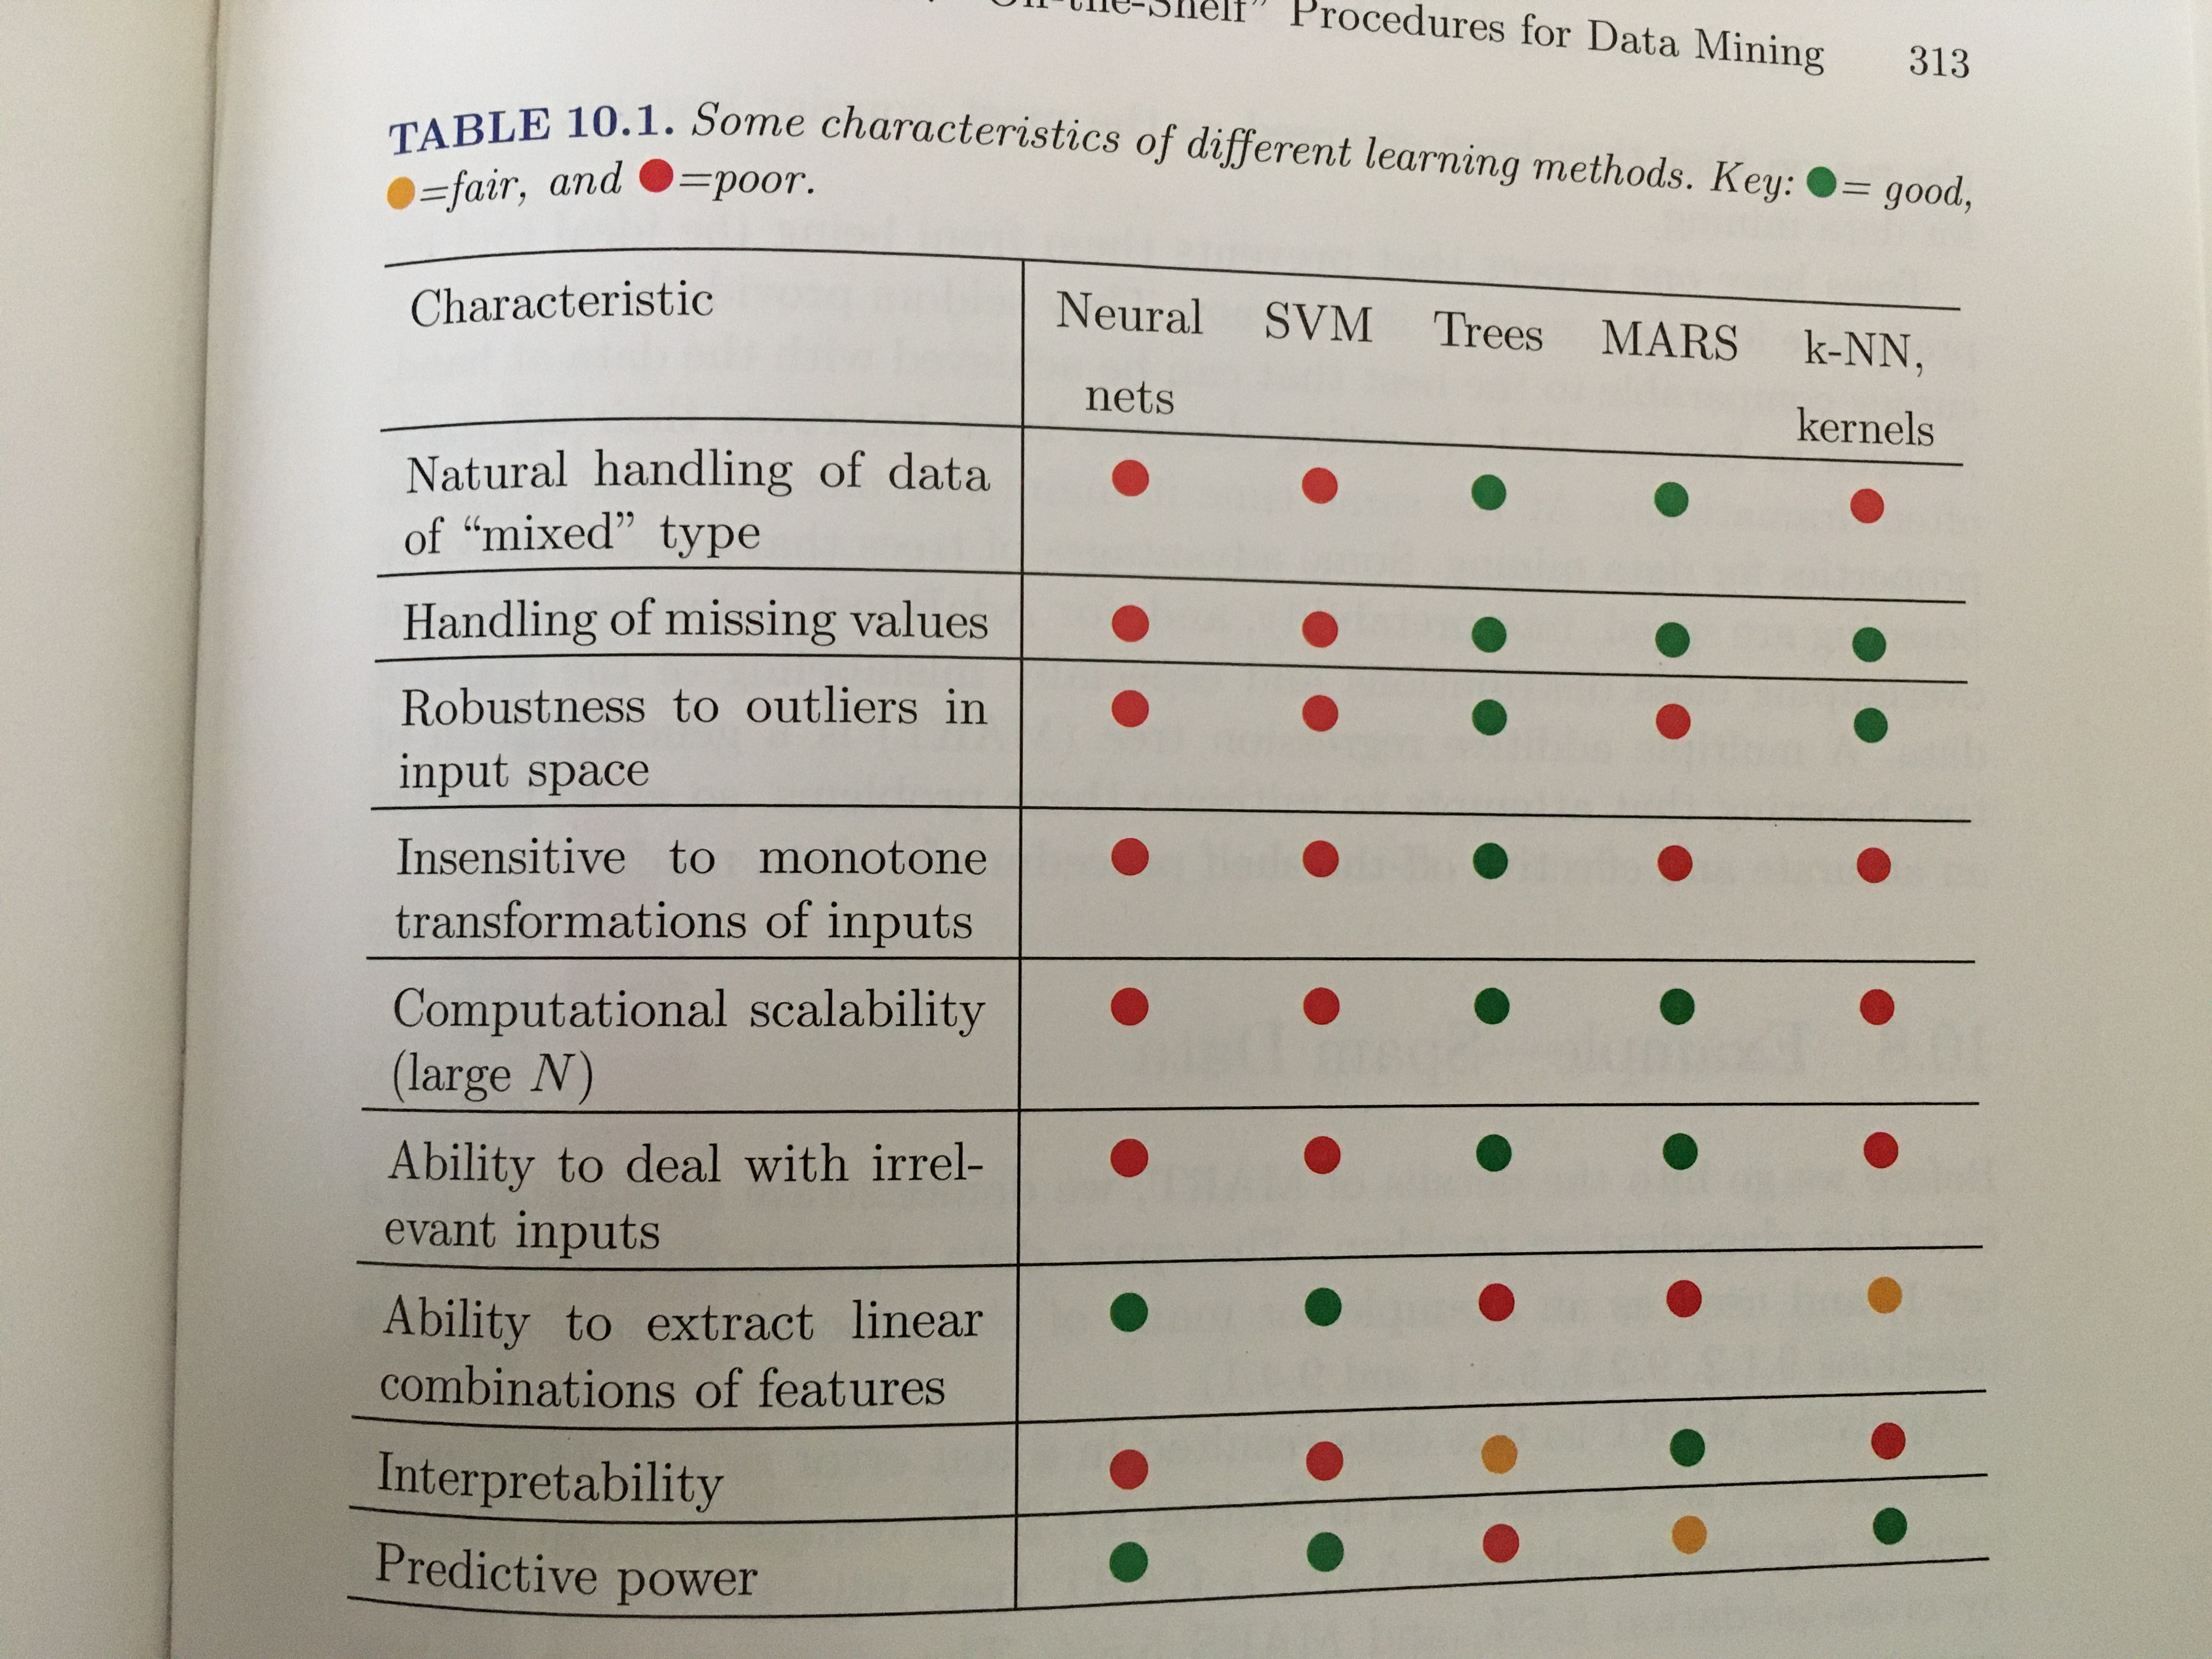
\includegraphics[scale=0.05]{../../Figures/fig_comparison.png}
		\end{figure}
	\end{frame}
	
	\begin{frame}{References}
		
		Materials and some of the pictures are from (1),(2), and (3).
		\begin{enumerate}
			\item Gareth James et al. {\it An Introduction to Statistical Learning with applications in R}. Springer (2015)
			\item Trevor Hastie et al. {\it The Elements of Statistical Learning } Springer (2001). 
			\item Aur\'elien G\'eron. {\it Hands-on Machine Learning with Scikit-Learn \& TensorFlow} O'Relly (2017)
			
		\end{enumerate}	
		
		I have used some of the graphs by hacking TiKz code from StakExchange, Inkscape for more aesthetic plots and other old tricks of \TeX
	\end{frame}	
	
	
\end{document}